\documentclass[12pt]{article}
\usepackage[english]{babel}
\usepackage[utf8x]{inputenc}
\usepackage[T1]{fontenc}
\usepackage{scribe}
\usepackage{listings}
\usepackage{mathtools}
\usepackage{listings}
\usepackage{tikz}
\usepackage{xcolor}


\lstdefinestyle{mystyle}{
    backgroundcolor=\color{backcolour},   
    commentstyle=\color{codegreen},
    keywordstyle=\color{magenta},
    numberstyle=\tiny\color{codegray},
    stringstyle=\color{codepurple},
    basicstyle=\ttfamily\footnotesize,
    breakatwhitespace=false,         
    breaklines=true,                 
    captionpos=b,                    
    keepspaces=true,                 
    numbers=left,                    
    numbersep=5pt,                  
    showspaces=false,                
    showstringspaces=false,
    showtabs=false,                  
    tabsize=2
}

\tikzstyle{data} = [circle, minimum size = 3 cm,text centered, draw=black, thick, fill=red!30, text=white]
\tikzstyle{model} = [rectangle, minimum width=3cm, minimum height=3cm, text centered, draw=black, fill=orange!30]
\tikzstyle{arrow} = [thick,->,>=stealth]
\tikzstyle{outp} = [rectangle, rounded corners, minimum width=3cm, minimum height=3cm,text centered, draw=black, fill=green!30]

\Scribe{Group 23 \& 24}
\Lecturer{Abir De}
\LectureNumber{12}
\LectureDate{March 1, 2023}
\LectureTitle{Convexity, Dual Formulation and Similarity Measure}

\lstset{style=mystyle}

\begin{document}
	\MakeScribeTop
\section{Introduction}
Till now, we have seen that original problem of SVM is given by
\begin{gather*}
    \min_{\boldsymbol{w},\; b} \lambda||\boldsymbol{w}||^2 + c\sum_{i \in \mathcal{D}}( 1 - (y_i(\boldsymbol{w}^T\boldsymbol{x_i}+b))
\end{gather*}
This is a convex problem since its double derivative is a matrix with positive eigenvalues. 
\begin{gather*}
    \begin{aligned}\frac{\partial \lambda||\boldsymbol{w}||^2 }{\partial \boldsymbol{w}}= 2 \lambda \boldsymbol{w} \\
    \frac{\partial ^2 \lambda||\boldsymbol{w}||^2 }{\partial \boldsymbol{w}^2}  = 2 \lambda I_{d x d}
     \end{aligned}
\end{gather*}
Here $||\boldsymbol{w}||^2$ is norm of the vector $\boldsymbol{w}$, so its derivative is a vector and the double derivative is a square matrix of dimension d.
Since $\lambda$ is positive, the double derivative will be positive and hence it becomes a convex optimization problem.

\section{Convexity of Dual Formulation problem}
The optimization problem for the dual formulation of SVM is given by 
\begin{gather*}
    \max_{\boldsymbol{\alpha}} \sum_{i \in \mathcal{D}} \alpha_i - \frac{\sum_{i,j} \alpha_i \alpha_j y_i y_j {x_i}^T x_j }{2 \lambda} \\
    \intertext{where,}
     \sum_{i \in \mathcal{D}} \alpha_i y_i = 0 \\
     0 \leq \alpha_i \leq C
\end{gather*}
Consider
\begin{gather*}
  G(\boldsymbol{\alpha}) = \sum_{i \in \mathcal{D}} \alpha_i - \frac{\sum_{i,j} \alpha_i \alpha_j y_i y_j {x_i}^T x_j }{2 \lambda}
\end{gather*}
Like the original problem of SVM, here also the double derivative of $G(\boldsymbol{\alpha})$ will be a matrix whose $ij^{th}$ entry is given by
\begin{gather*}
    [\frac{\partial ^2 G(\boldsymbol{\alpha}) }{\partial \boldsymbol{\alpha}^2} ]_{(i,j)} = -\frac{y_i y_j {x_i}^T x_j }{2 \lambda}
\end{gather*}
Since each element contains $y_i y_j (\boldsymbol{x}_i \cdot\boldsymbol{x}_j)$ , interchanging i and j gives same element, means it is a symmetric matrix. Also all entries are real numbers so it is a real symmetric matrix. 
\newline Further, we can represent $G(\alpha)$ as 
 \begin{gather*}
  G(\boldsymbol{\alpha}) = \sum_{i \in \mathcal{D}} \alpha_i +{\boldsymbol{\alpha}}^T\frac{\partial ^2 G(\boldsymbol{\alpha}) }{\partial \boldsymbol{\alpha}^2}\boldsymbol{\alpha}
\end{gather*}
The matrix $\frac{\partial ^2 G(\boldsymbol{\alpha}) }{\partial \boldsymbol{\alpha}^2}$ has negative eigenvalues so the optimization for the dual formulation of SVM becomes a concave optimization problem. Hence we focus on maximizing $G(\boldsymbol{\alpha})$ here. While the original problem of SVM was a convex optimization problem, hence we minimized the function there.




\section{Problem with Dual}

While using dual, we have n variables ($\alpha_1,\alpha_2,\alpha_3,...$).
\newline
By comparison, the primal problem had d variables where $d \le n$.
\newline
Thus with n parameters of dimension d, to store we need memory of order $O(||d^2||)$.\\
i.e.
\begin{gather*}
   G(\Vec{\alpha}) = \sum_{i \in \mathcal{D}} \alpha_i +{\vec{\alpha}}^T\frac{\partial ^2 G(\Vec{\alpha}) }{\partial {\alpha}^2}\vec{\alpha} 
\end{gather*}
\\ 
Since double derivative has terms consisting of $y_i y_j (\boldsymbol{x}_i \cdot\boldsymbol{x}_j)$, the number of computations required will be of order $d^2$. And we can neither diagonalize because for that too, we will require to store the matrix first in the memory.
\\The solution to this problem is that we choose a random variable $\boldsymbol{w}$ from some random distribution, perform mixing on it with $\boldsymbol{\alpha}$, and build a new function $\hat{G(\boldsymbol{\alpha})}$ such that the expectation of $\hat{G(\boldsymbol{\alpha})}$ over $\boldsymbol{w}$ equals to G($\boldsymbol{\alpha})$.
\begin{gather*}
   \hat{G(\boldsymbol{\alpha})} = g(\boldsymbol{w},\boldsymbol{\alpha})\\
    \mathbb{E}_{\boldsymbol{w}}[\hat{G(\boldsymbol{\alpha})}] = G(\boldsymbol{\alpha})
\end{gather*}


\newpage
\section{Similarity measure}
The w can be represented in terms of $\boldsymbol{\alpha}$ as

\begin{gather*}
   w = \frac{\sum_i \alpha_i y_i x_i}{2\lambda}
   \intertext{Also, remember that}
   \sum_i \alpha_i y_i = 0
   \intertext{For example, take}
       \hat{y} = sign(\boldsymbol{w}^T\boldsymbol{x}+b)
   \\ \hspace{2.1 cm}= sign(\frac{\sum_{i,j} \alpha_i y_i {x_i}^T x_j}{2\lambda}+b)   
\end{gather*}

Here we are checking the similarity of x by doing ${x_i}^T x_j$ and then weighting similarity by $y_i$ first and then again weighting it by $\alpha_i$ since $\sum_i \alpha_i y_i = 0$. So we are taking the weighted average of similarities. 

\par But for correctly classified points, $\alpha_i$ = 0. So we are only observing misclassified points and points lying on the hyperplane. It sounds counter-intuitive since we are observing only misclassified points and points lying on hyperplane instead of correctly classified points.
\par Another strategy can be that we check the neighborhood and take the average of the labels. In this strategy, we will get correct result for good points but the wrong result for bad points.
\par We want a unified strategy for all points. So will use the similarity measure strategy. Even if we are looking at misclassified/ boundary points only, it will take us max to the boundary only but it is fine since it also works for bad points. 
\par So even though we are more confident in neighborhood checking method for good points, we use similarity measure method to get a uniform strategy for bad points as well. 

\begin{figure}[htp]
    \centering
    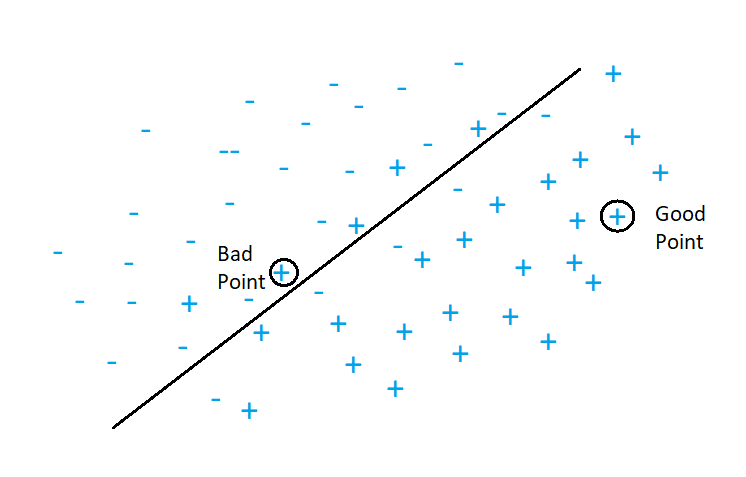
\includegraphics[scale=0.55]{nh.png}
\end{figure}






\newpage
\subsection*{similarity measure for a special case}
Consider the dataset shown in the figure below.
 \begin{figure}[htp]
    \centering
    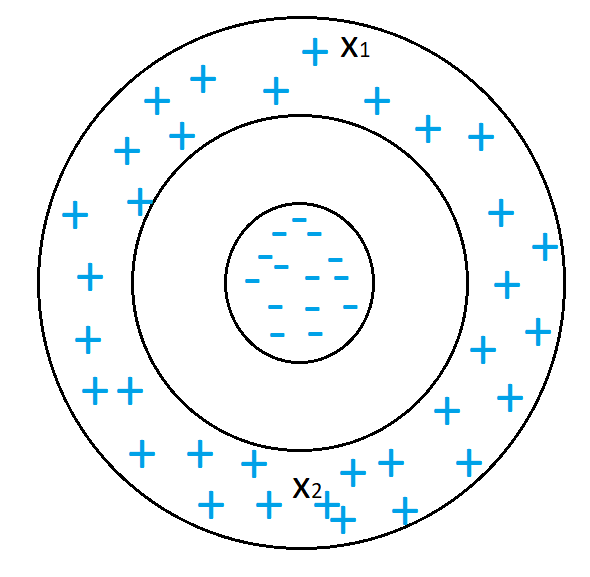
\includegraphics[width=7cm]{smsc.png}
\end{figure}

As shown in the figure, the region containing '-' points is completely surrounded by the region containg '+' points. Consider two points $x_1$ and $x_2$ in the outer region.
Now we have 2 choices for similarity measure.
\begin{gather*}
 (i): sim(x_1,x_2) \propto -|| x_1 - x_2 ||
 \intertext{or}
(ii): sim(x_1,x_2) \propto -|\hspace{1mm} || x_1|| - ||x_2 ||\hspace{1mm}|
\end{gather*}
\par In this case, the distance from the origin is a more convenient measure of similarity; hence the second choice is better here.  While in the first choice, it is directly taking the distance between two points. So if you consider points $x_1$ and $x_2$ of the diagram, although they are similar, the choice (i) of similarity will fail there. But as far as the purpose of SVM is concerned, choice (i) can also work as our similarity measure since we will be observing the nearest points only. 
\end{document}
